\documentclass[aps,prl,twocolumn,
	groupedaddress,superscriptaddress,
	amsfonts,amssymb,amsmath,floatfix,
	citeautoscript]{revtex4-1}

\usepackage{graphicx}
\usepackage[centering,hmargin=20mm,tmargin=30mm,bmargin=25mm]{geometry}
\usepackage{multirow}
\usepackage{newtxtext}
\usepackage[cmintegrals]{newtxmath}

%----- References -----
\usepackage{xcolor}
\usepackage{hyperref}
\hypersetup{colorlinks,
	linkcolor={blue!75!black!80!yellow},
	citecolor={blue!75!black!80!yellow},
	urlcolor={blue!75!black!80!yellow}
}

%----- Captions in sans font -----
\makeatletter
\renewcommand\@make@capt@title[2]{%
	\@ifx@empty\float@link{\@firstofone}{\expandafter\href\expandafter{\float@link}}%
	\sffamily{\textbf{#1}}\@caption@fignum@sep#2
}%
\renewcommand\figurename{Fig.}
\makeatother

\thickmuskip=5mu plus 2mu minus 1mu  %binary relations (default, 5mu plus 5mu)
\medmuskip=4mu plus 2mu minus 2mu    %binary operations (default, 4mu plus 2mu minus 4mu)

\frenchspacing %Ensure that revTeX does not do "double spaces" after punctuation

\renewcommand{\Im}{\operatorname{Im}}
\renewcommand{\Re}{\operatorname{Re}}
\newcommand{\sub}[1]{\ensuremath{_{\textrm{#1}}}} %Upright multi-character subscript
\newcommand{\super}[1]{\ensuremath{^{\textrm{#1}}}} %Upright multi-character superscript

\newcommand{\HarvardSEAS}{John A. Paulson School of Engineering and Applied Sciences, Harvard University, Cambridge, MA, USA}
\newcommand{\MITPhy}{Department of Physics, Massachusetts Institute of Technology, Cambridge, MA, USA}

\usepackage[normalem]{ulem}
\newcommand{\Jadd}[1]{\textcolor{blue}{#1}}
\newcommand{\Jrem}[1]{\textcolor{blue}{\sout{#1}}}


%\usepackage[usenames]{color}
%\newcommand{\edited}[1]{{\color{red} #1}}

\begin{document}

\title{Variational theory of the ground state of quantum electrodynamics}

\author{Nicholas Rivera}\email{nrivera@seas.harvard.edu}\affiliation{\HarvardSEAS}\affiliation{\MITPhy}
\author{Johannes Flick}\email{flick@seas.harvard.edu}\affiliation{\HarvardSEAS}
\author{Prineha Narang}\email{prineha@seas.harvard.edu}\affiliation{\HarvardSEAS}


\date{\today}

\begin{abstract}
The past decade has brought rapid theoretical and experimental advances in the field of ultra-strong coupling of light and matter from microwave to optical frequencies. Many of the theoretical analyses of such systems proceed by considering simple two-level systems coupled to a single cavity mode. There remains a need to understand light-matter coupling  in contexts of complicated electronic systems coupling to many-mode or continuum photonic systems, as well as a need to understand how vacuum fluctuations of electromagnetic fields are altered in real space by strong light-matter coupling in such complex systems.  In this work, we develop a variational theory of the ground state of a quantum electrodynamical system of coupled light and matter. Essential to our ansatz is the notion an effective photonic vacuum whose modes are different than the modes in the absence of light-matter coupling. Our variational formulation leads to a set of general equations that can describe the ground state of multi-electron systems coupled to many photonic modes in real space. As a first step towards an  \textit{ab initio} approach to ground states in QED, we apply our ansatz to a Rabi model involving a multi-level emitter with many optical modes, a model which cannot be analytically solved. We find a compact semi-analytic formula which describes the ground state energy very accurately (to less than 1\% error) in all regimes of coupling parameters allowed by the Thomas-Reiche-Kuhn sum rule. We expect our method to give rise to highly accurate descriptions of ground-state phenomena in quantum electrodynamics in complicated systems, such as Casimir forces, Lamb shifts, and fluctuational electrodynamics phenomena. 
\end{abstract}

\maketitle

%\section{Introduction}
%\label{sec:Introduction}

The past decade has brought an explosion of effort and experimental progress in realizing the coupling of matter and quantized electromagnetic fields beyond a regime of weak coupling, in which perturbative treatments of quantum electrodynamical couplings can no longer accurately describe the dynamics \cite{flick7strong,ruggenthaler2017b,forn2018ultrastrong,kockum2018ultrastrong}. Ultra-strong, or even deep-strong coupling is now regularly observed in superconducting qubits at microwave frequencies \cite{blais2004,wallraff2004,yoshihara2017superconducting,forn2017ultrastrong}, ensembles of molecules in optical cavities \cite{hutchison2012,hutchison2013,coles2014,coles2014b,shalabney2015coherent, thomas2016,ebbesen2016}, 2D electron gas cyclotron resonances coupled to cavities \cite{hagenmuller2010ultrastrong,scalari2012ultrastrong,zhang2016collective}, intersubband transitions in quantum wells coupled to cavities \cite{todorov2010ultrastrong,geiser2012ultrastrong}, and single-emitters in ultra-confined plasmonic geometries \cite{benz2016,chikkaraddy2016}. Proposals for new platforms of ultra-strong coupling include emitters coupling to highly confined polaritons in metals and polar insulators \cite{rivera2016shrinking}, highly ionized atoms coupled to optical media via the Cerenkov effect, and many more. The proposed applications for ultra- and deep-strong coupling of light and matter are similarly broad, including simulation of many-body systems \cite{forn2018ultrastrong}, altering chemical reactivity~\cite{hutchison2012, thomas2016,flick2017} and electronic transport properties \cite{orgiu2015}, realizing analogues of nonlinear optical processes with vacuum fluctuations \cite{kockum2017deterministic}, and even as new sources of photons through the dynamical Casimir effect \cite{ciuti2005quantum}.

In the nonperturbative regime of quantum electrodynamics, there are very few models which can be analytically solved. In particularly, the only exactly solvable models in all regimes of coupling parameters include the Rabi model~\cite{braak2011}, which describes the coupling of a two-level atom to a single mode, the Hopfield model \cite{hopfield1958theory}, which describes the coupling of a harmonic oscillator to any number of cavity modes, and Dicke models based on two-level systems and harmonic oscillators \cite{dicke1954coherence}. Any realistic system which deviates from these simpler models require numerical diagonalization approaches for an exact solution, which become unwieldy when the dimension of the electronic Hilbert space becomes large, as is the case when describing an electronic system in real space. It also becomes unwieldy when one needs to keep track of many cavity modes which can also be populated with many photons. Exciting new developments towards ab-initio studies of QED have proceeded by proposing reduced-quantity descriptions such as density-functional descriptions of the light-matter coupling \cite{ruggenthaler2014,pellegrini2015,flick2015,dimitrov2017,flick2018,flick2018b,schaefer2018}. With such density-functional descriptions, workers in this field have been able to compute ground-state and time-dependent properties of realistic molecules in optical cavities \cite{flick2017c}. 

In what follows, we propose the use of variational methods for the solution of \emph{ab initio} QED problems.  In particular, we develop an ansatz in which the ground state can be considered as a factorizable state of an effective matter and effective photon quasiparticle both in their respective ground states. This ansatz, reminiscent to the Hartree-Fock ansatz of electronic structure theory, leads to coupled eigen-equations describing the ground-state of the light-matter system. We benchmark our ansatz against a multi-level and multi-mode Rabi model parameterized by the strength of the characteristic momentum matrix elements describing the coupling of the matter and the electromagnetic fields. We find that for light-matter couplings that respect the Thomas-Reiche-Kuhn sum rule, our theory finds the ground state energy to a remarkable accuracy of more than >99\%, even in non-perturbative coupling regimes.  In regimes where our results are accurate, we claim we have found the effective quasiparticle description of the ground state. Moreover, in this regime, the ground state interaction energy manifests itself as the difference in zero-point energies between the quasiparticles and the bare particles.  Our findings furnish a non-perturbative theory of the Lamb shift, allowing us to non-perturbatively calculate position-dependent Lamb shifts of ground and excited states that give rise to Casimir-Polder forces.

%Our results service several aims. First, they suggest a novel variational approach for understanding ground states in ultra-strongly coupled light-matter systems. Second, they provide a general framework for understanding light-matter decoupling effects in the regime of strong light-matter interactions. Third, they prove a non-perturbative theory of Casimir-Polder forces \Jadd{(cite)}. Finally, they provide a rigorous concept of correlation energy in quantum electrodynamics in a way analogous to electronic structure theory. 

%The outline of this work is as follows: in section~\ref{sec:variational_ansatz}, we develop the variational ansatz for the ground state of the Hamiltonian of macroscopic quantum electrodynamics. In section~\ref{sec:multi-level}, we calculate the ground state energy according to this ansatz for the multi-level and multi-mode Rabi model and compare it to numerical diagonalization of the same problem. In Section~\ref{sec:extensions}, we propose a self-consistent extension of our ansatz. 

The QED Hamiltonian takes the form $H = H_{mat}+H_{em}+H_{int}$ where $H_{mat}$ describes the matter in the absence of the quantized electromagnetic field, $H_{em}$ describes the photons in the absence of the matter, and $H_{int}$ describes the coupling between light and matter. The matter Hamiltonian takes the form:
\begin{align}
H_{el} &= \int d^3x ~\psi^{\dagger}(x)\left(-\frac{\hbar^2\nabla^2}{2m} + v_{ext}(x) \right)\psi(x) \nonumber \\ &+ \frac{1}{2}\int d^3x d^3x'~ \psi^{\dagger}(x)\psi^{\dagger}(x')V(x-x')\psi(x')\psi(x),
\end{align}
where $v_{ext}$ is the one-body potential, $V(x-x')$ is the two-body interaction kernel, and $\psi$ is the second-quantized electron field. %\Jadd{(shouldn't x also be bold when it is an argument, since it a vector)}

Parameterizing the electromagnetic field purely in terms of a vector potential: $\mathbf{E} = -\partial_t\mathbf{A}$ and $\mathbf{B} = \nabla\times\mathbf{A}$. This renders the free electromagnetic Hamiltonian as
\begin{equation}
H_{em} = \int d^3x~ \epsilon (\partial_t \mathbf{A}(x))^2 + \mathbf{A}(x)\cdot(\nabla\times\mu^{-1}\nabla\times\mathbf{A}(x)),
\end{equation}
where $\epsilon$ and $\mu$ represent a non-dispersive and positive dielectric and magnetic background that the matter and photon occupy. For cases we consider in this work, these will be taken to be unity, but we leave them here for the sake of generality.

The interaction Hamiltonian takes the form:
%\begin{align}
%H_{int} = &\frac{-i\hbar e}{2m}\int d^3x ~\psi^{\dagger}(x)(\mathbf{A}\cdot\nabla +  \nabla \cdot \mathbf{A})\psi(x) + \nonumber \\ &\frac{e^2}{2m}\int d^3x ~\psi^{\dagger}\psi\mathbf{A}^2(x).
%\end{align}
\begin{align}
H_{int} &= \frac{-i\hbar e}{2m}\int d^3x ~\psi^{\dagger}(x)(\mathbf{A}(x)\cdot\nabla +  \nabla \cdot \mathbf{A}(x))\psi(x) \nonumber \\ &+ \frac{e^2}{2m}\int d^3x ~\psi^{\dagger}(x)\psi(x)\mathbf{A}^2(x).
\end{align}

This Hamiltonian, which depends on the fields $\psi$ and $\mathbf{A}$ can be parameterized in terms of an orthonormal set of electron single-particle wavefunctions $\{\psi_n\}$, and in terms of a set of photonic mode functions $\{\mathbf{F}_i\}$ via mode expansions for the electronic and photonic field operators. The electron field operator takes the form $\psi(x) = \sum_n \psi_n(x)c_n$.
In this second-quantized description, the $c_n$ is an annihilation operator for an electron corresponding to state $n$. The electromagnetic field operator takes the form $\mathbf{A}(x) = \sum_i\sqrt{\frac{\hbar}{2\epsilon_0\omega_i}} \left(\mathbf{F}_i(x)a_i+\mathbf{F}^*_i(x)a^{\dagger}_i\right)$. In the electromagnetic field operator, we parameterize not only by the mode functions but also by modal frequencies. We have chosen a form for the vector potential operator which mirrors the choice generally adopted in QED. The normalization chosen for the electron wavefunctions is $\int d^3x~ \psi_m^*\psi_n = \delta_{mn}$ while for the photon mode functions, it is $\int d^3x~\epsilon\mathbf{F}_i^*\cdot\mathbf{F}_j = \delta_{ij}.$

With the Hamiltonian set up, we now move to describe a variational theory of the ground state. In the variational theorem, we choose some ansatz $|\Omega\rangle$ for the ground state of $H$. The variational theorem ensures that $\langle \Omega|H|\Omega\rangle$ is an upper bound for the ground state energy. Parameterizing the ground state to generate a family of ground states, and minimizing $\langle \Omega|H|\Omega\rangle$ with respect to the introduced parameters gives the best upper bound for the ground state energy for the chosen family of ground states.  We choose as our ansatz
\begin{equation}
|\Omega\rangle = \left( \prod\limits_n c_n^{\dagger}|0_n\rangle,\right) \otimes \left(\bigotimes_i|0_i\rangle\right),
\end{equation}
In such an ansatz, $\prod\limits_n c_n^{\dagger}|0_n\rangle$ represents a "filled Fermi sea" for effectively non-interacting electrons, and $|\phi\rangle$ represents a "photonic vacuum" for effectively non-interacting photons. Implicitly, this ansatz, once we take the expectation value $\langle \Omega|H|\Omega\rangle$, denotes a family of ansatzes labeled by all the possibilities for the electron wavefunctions and photon mode functions. Thus, we shall minimize the expectational value with respect to $\psi_n, \psi_n^*, \mathbf{F}_i, \mathbf{F}_i^*$, and $\omega_i$. Note that the electromagnetic field gets two sets of (distinct) variational parameters, $\omega_i$ and $\mathbf{F}_i$. The last thing to note before taking the expectation values and minimization is that we should focus on the submanifold of variations that keep the complete set of electron and photon functions normalized. This shall be enforced by constructing the Lagrange function:
\begin{widetext}
\begin{equation}
\mathcal{L}[\{ \psi_n,\psi_n^* \},\{ \mathbf{F}_i,\mathbf{F}_i^*,\omega_i \}] = \langle \Omega |H|\Omega\rangle - \sum_n E_n\left(\int d^3x ~\psi_n^*\psi_n - 1 \right) - \sum_n \frac{\hbar\lambda_i}{2}\left(\int d^3x ~\epsilon\mathbf{F}_i^*\cdot\mathbf{F}_i - 1 \right),
\end{equation}
\end{widetext}
with the $E_n$ and $\lambda_i$ being the Lagrange multipliers that enforce the normalization condition. Evaluating the expectation value of the Hamiltonian, and minimizing the Lagrange function  with respect to the orbitals, photon modes, and photon frequencies, immediately yields:
\begin{align}
&\left(\frac{\mathbf{p}^2}{2m}+v_{ext}(x) \right)\psi_i(x) + \nonumber \\ &\sum\limits_{j=1}^N \int d^3x' ~ V(x-x')\psi^*_j(x')\psi_j(x')\psi_i(x) \nonumber \\ & - \sum\limits_{j=1}^N \int d^3x' ~ V(x-x')\psi_j(x')\psi_j(x)\psi_i(x')  \nonumber \\ &+ \frac{\hbar e^2}{4m\epsilon_0}\sum_n \frac{1}{\omega_n}|\mathbf{F}_n|^2\psi_i(x)   = E_i\psi_i(x).
\end{align}
for the electron orbitals and energies. One sees that in addition to the one-body and Hartree-Fock terms for the electrons, the effect of the QED coupling is to add a one-body ponderomotive potential. We note that in the often used dipole approximation, the ponderomotive potential has no effect as it becomes independent of position.
\begin{figure}[t]
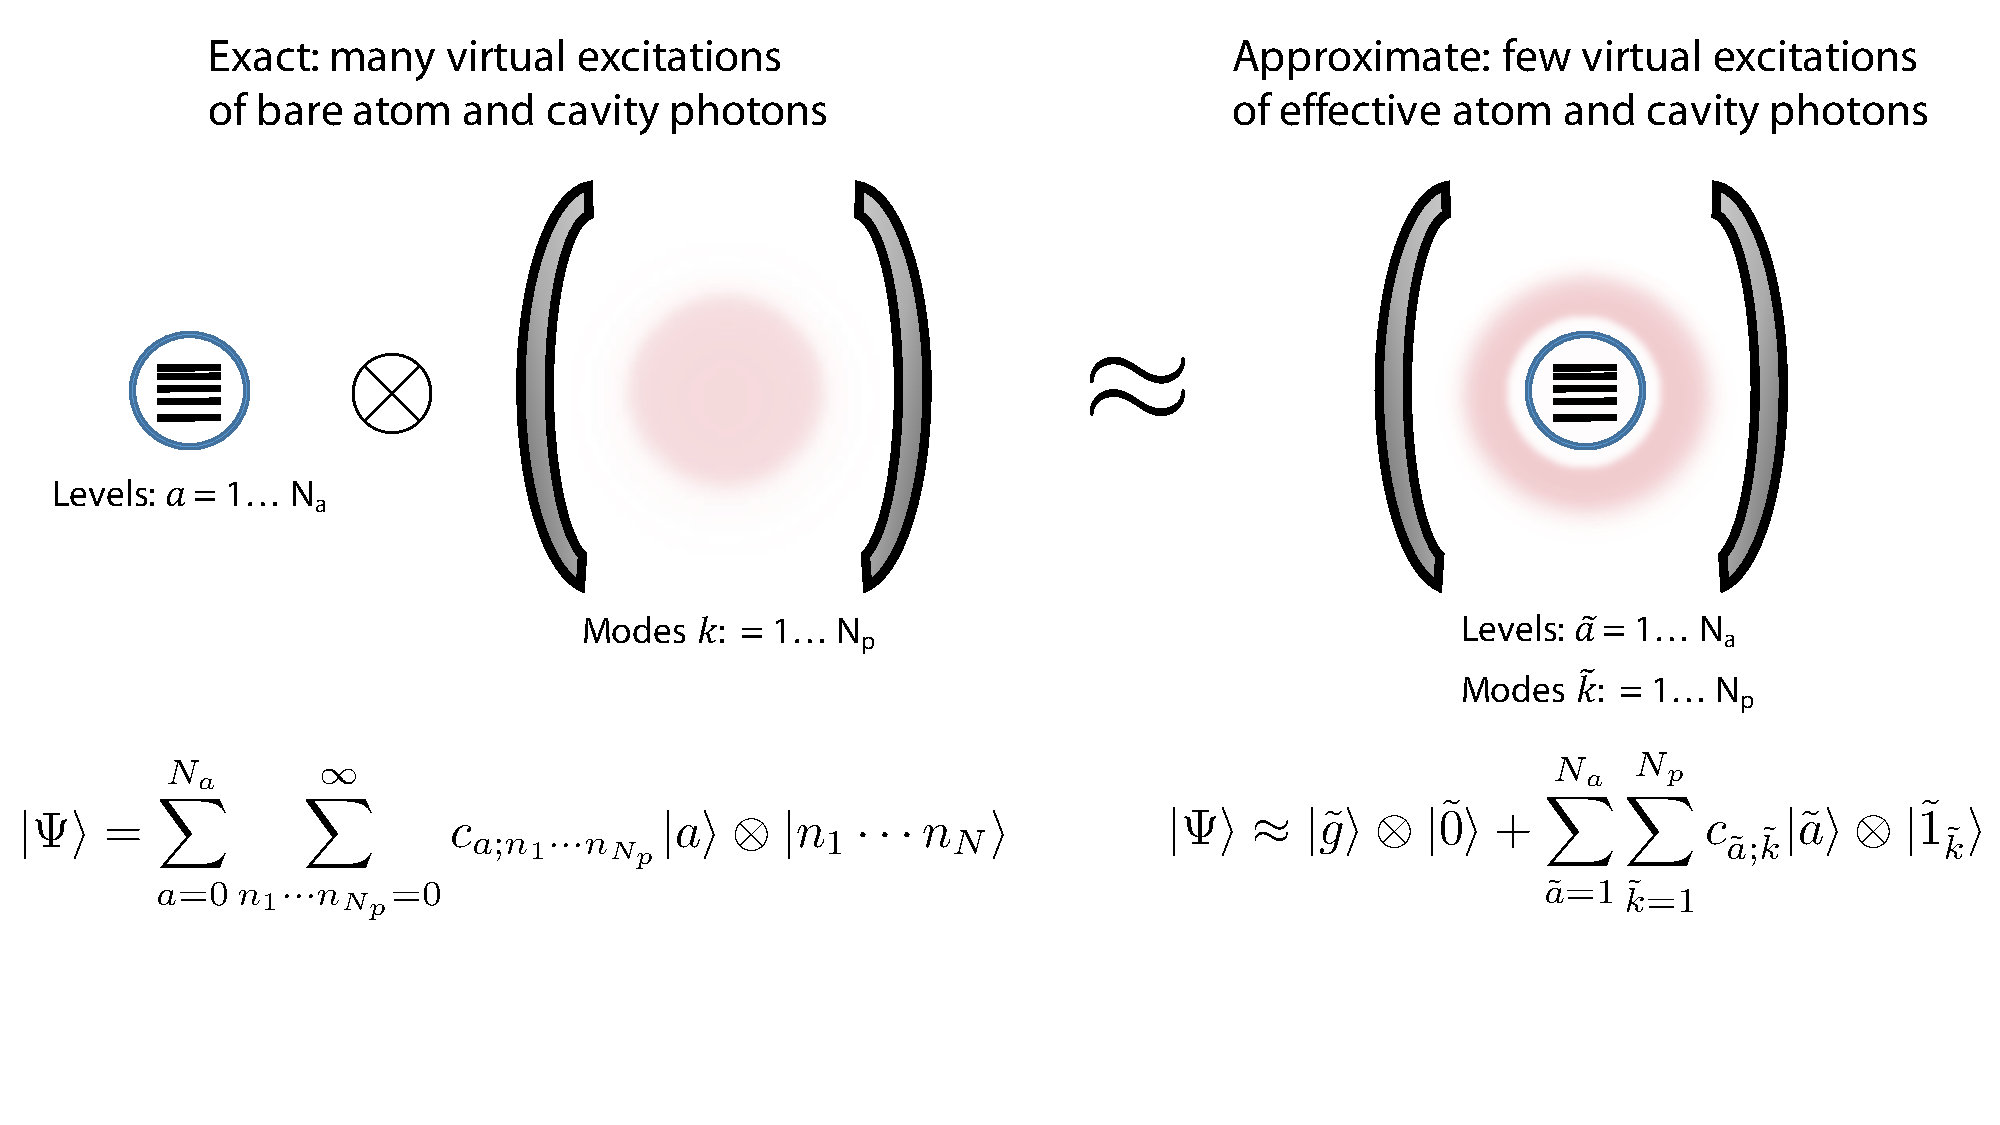
\includegraphics[width=8.5cm]{conceptfigure.pdf}
\caption{\textbf{Ground-state ansatz applied to matter in a cavity: effectively decoupled matter and photons.} (Left) Bare description of the coupled light-matter ground state in terms of many virtual excitations of the emitter state and the bare cavity photons. (Right) Quasiparticle description of the coupled system as a factorable state an effective emitter in its ground state and the vacuum of an effective photonic degree of freedom.}
\label{fig:ansatz}
\end{figure}
For the photon orbitals and energies, the minimization yields:
\begin{equation}
\left( \nabla\times\nabla\times - \left(1-\frac{\omega_p^2}{\omega_q^2} \right)\right)\mathbf{F}_q = 0,
\end{equation}
where $\omega_p^2 = \frac{e^2}{m\epsilon_0}\sum\limits_{i=1}^N |\psi_i(x)|^2$ is a position-dependent squared-plasma frequency which will push the photon orbitals out of the region where the emitter is located.

Immediately, one notices that the term in the interaction Hamiltonian linear in the vector potential makes no contribution to the expectation value of the ground state of the energy in this ansatz. In many quantum electrodynamical problems, this linear term, which has zero expectation value in our ansatz, is important. To first order, it leads to spontaneous emission of a single photon. To second order, it leads to two (virtual) photon processes, such as van der Waals / Casimir-Polder forces on emitters, real photon processes such as two-photon emission, and effective interactions betweeen distinct emitters. Thus, we seek to capture the effect of this term. Physically, this term will mix the factorizable ground state of Equation (7) with terms that have virtual excitations of the matter, as well as virtual excitations of the electromagnetic field. The resulting state is now non-factorizable and we thus conclude that the term in the Hamiltonian linear in the vector potential leads to \textit{correlations} in the system, and contributes wholly at lowest order to the correlation energy of the quantum electrodynamical ground state.
\begin{figure}[t]
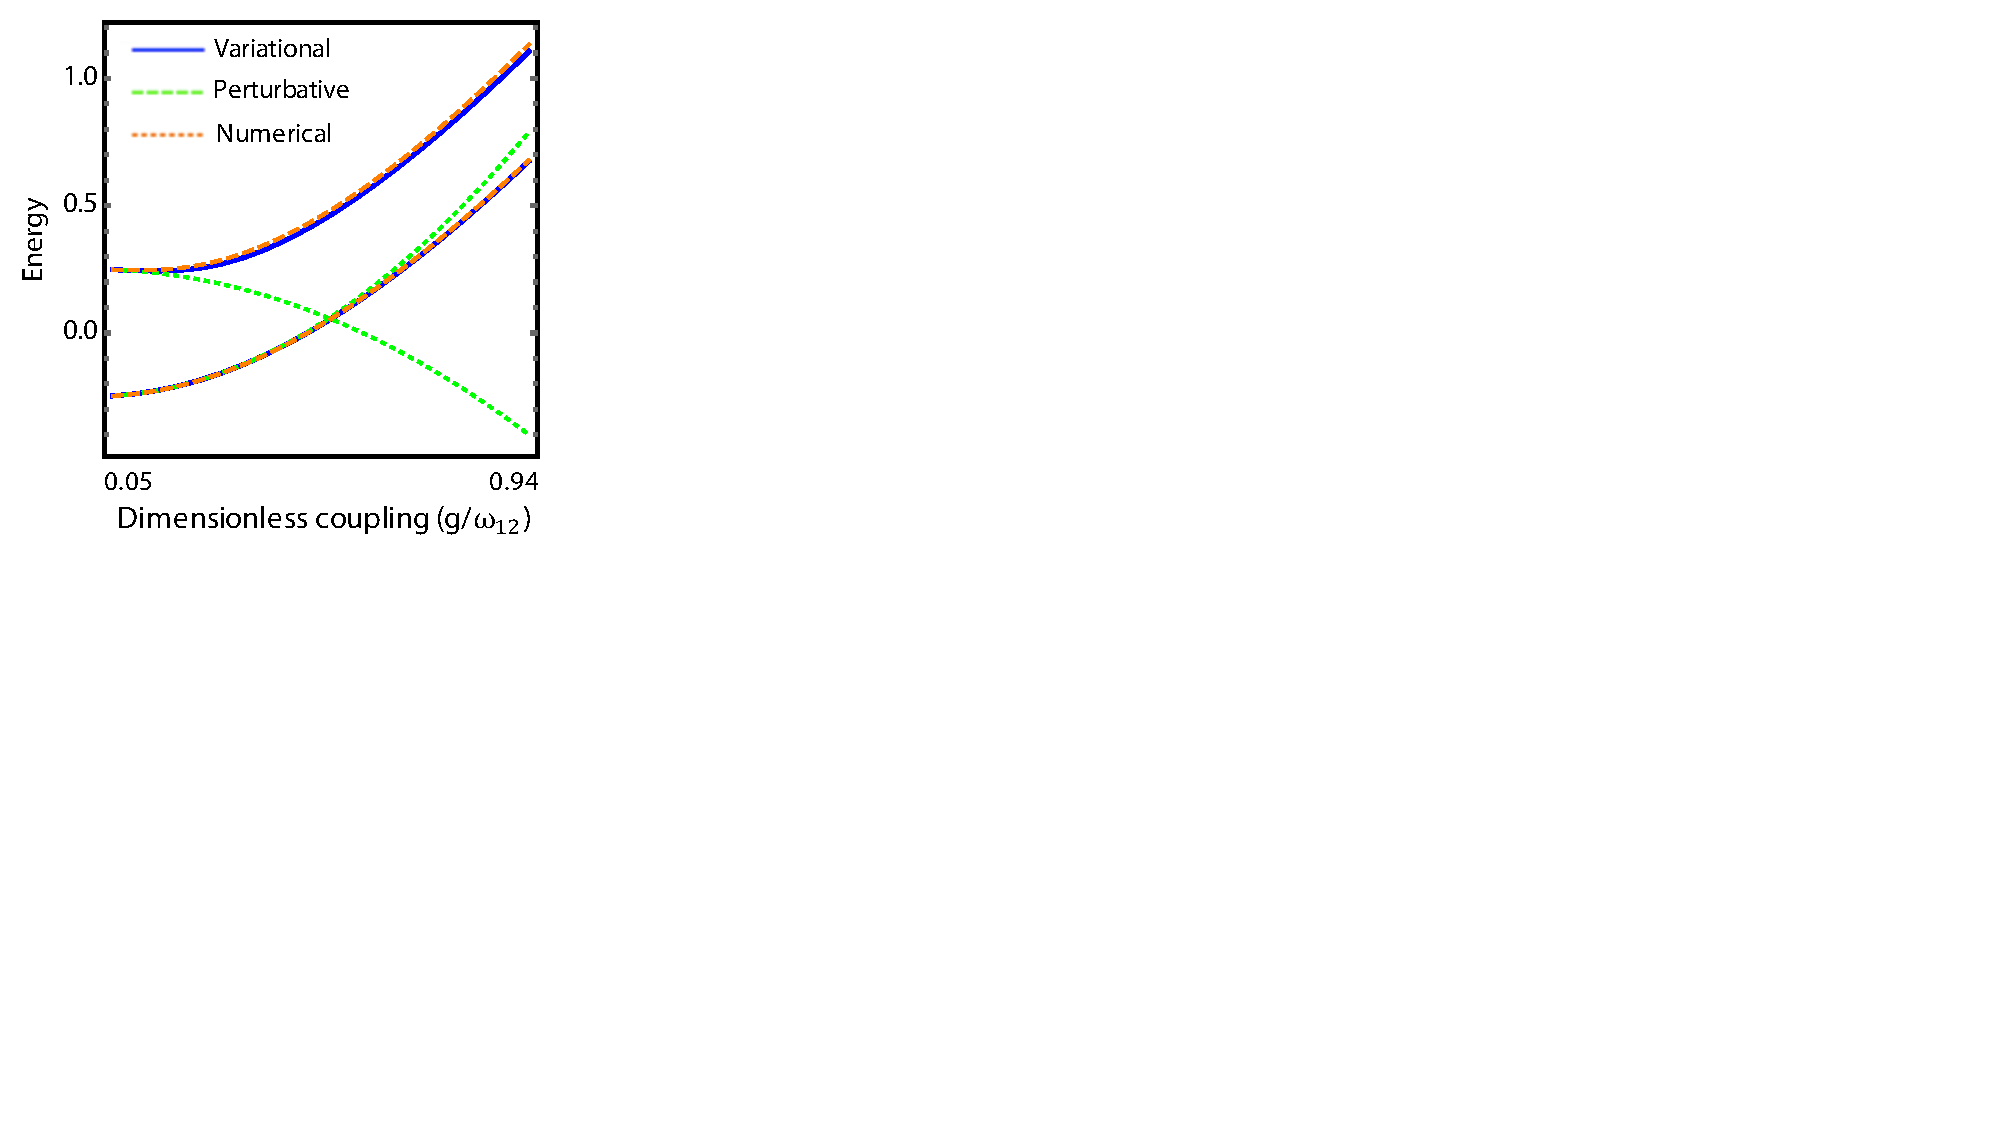
\includegraphics[width=5cm]{figure2new.pdf}
\caption{\textbf{Variational theory of ground and excited states in the ultra-strong coupling regime of QED.} Lowest two eigenvalues as a function of coupling for the multi-mode Rabi model describing the coupling of an emitter to a one-dimensional cavity. The variational results (blue) agree to within roughly a percent with the result derived by numerical diagonalization (orange) retaining up to four photons in the Hilbert space. The result from perturbation theory (green) disagrees strongly with the other methods of calculation for the first excited state due to a near-resonance between the bare transition energy and the bare lowest cavity mode.}
\label{fig:ansatz}
\end{figure}
We capture the effect of correlations perturbatively. In other words, we consider the second-order correction $\delta E$ to the ground state energy arising from the term in the Hamiltonian linear in the vector potential. That correction is given by 
\begin{equation}
\delta E = \frac{e^2\hbar^2}{8m^2\epsilon_0}\sum\limits_{q=1}^{N_p}\sum_{m=N_{\sigma}+1}^{\infty}\sum\limits_{1}^{N_{\sigma}} \frac{\Big| \int d^3x~\mathbf{F}_q^*\cdot\mathbf{j}_{nm}\Big|^2}{\omega_q(\omega_{mn} -\lambda_q)}
\end{equation}
where $\mathbf{j}_{nm} = \psi^*_n\nabla\psi_m - (\nabla\psi^*_n)\psi_m$, $\omega_{mn} = \omega_m - \omega_n$, $N_{\sigma}$ is the number of occupied orbitals, equal to the number of electrons (divided by 2 if spin is retained), and $N_p$ is the number of photon modes retained.  In a method without self-consistency, the electron and photon orbitals and eigenvalues are those obtained from Equations (6) and (7), and then the electron energies and orbitals as well as the photon frequencies and orbitals, are plugged into Equation (8).
\begin{figure}[t]
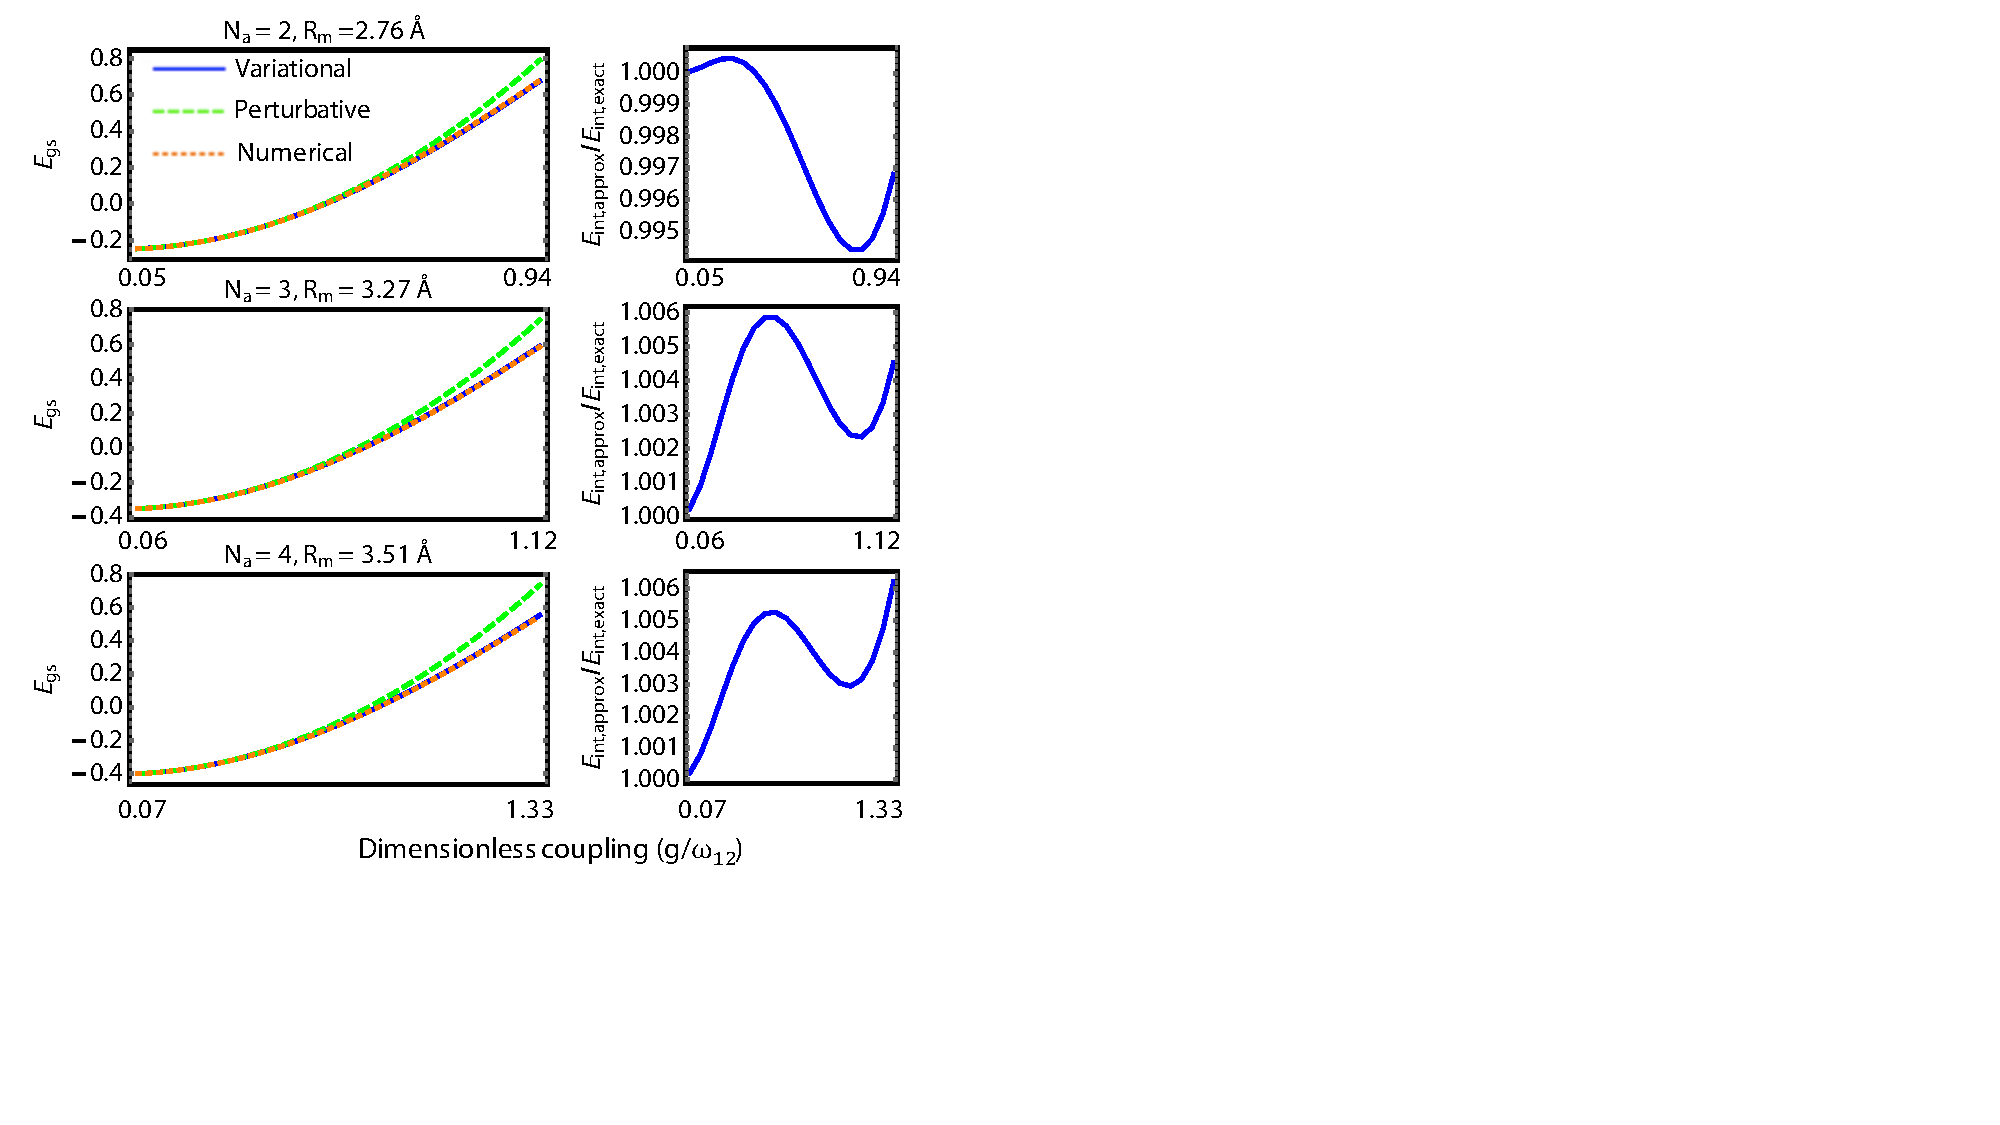
\includegraphics[width=8.4cm]{figure3new.pdf}
\caption{\textbf{Variational theory of ground state energy: accuracy as a function of number of emitter levels.} (Left) Ground-state energy of the one-dimensional multi-mode Rabi model as a function of the dimensionless coupling for two (top), three (middle), and four (bottom) level emitter systems with momentum matrix elements chosen to saturate the Thomas-Reiche-Kuhn sum rule. (Right) Ratio of the energy calculated with the variational theory and with numerical diagonalization. These results show that our accuracy is robust to the number of levels in the system. }
\label{fig:ansatz}
\end{figure}
In what follows, we provide a proof-of-concept demonstration of the efficacy of the variational theory derived here. We consider the QED Hamiltonian corresponding to a single emitter placed at position $z=d$ in a one-dimensional cavity oriented along the $z$-direction. As the cavity is considered for simplicity to be one-dimensional, the electric field is oriented along a single direction, denoted $x$, while the magnetic field is oriented along a direction transverse to both the electric field and the cavity length, denoted $y$.

Working under the long-wavelength or dipole approximation, the Hamiltonian can then be written as:
\begin{equation}\label{eq:hamiltonian}
H = H_{\text{matter}}+\frac{\epsilon_0}{2}\int dz~(E^2+c^2B^2)+\frac{q}{m}A(d)p + \frac{q^2}{2m}A^2(d).
\end{equation}
The fields can be expressed as a mode expansion via:
\begin{equation}\label{eq:mode_expansion}
A(z,t) = \sum\limits_{n=1}^{\infty} \sqrt{\frac{\hbar}{2\epsilon_0\omega_n }}(F_n(z)a_ne^{-i\omega_n t}+F^*_n(z)a_n^{\dagger}e^{i\omega_n t}),
\end{equation}
with $E(z,t) = -\partial_t A(z,t)$ and $B(z,t)=\partial_z A(z,t)$.  The $F_n(z)$ are the mode functions of the cavity, normalized such that $\int dz ~|F_n(z)|^2 = 1$. For a cavity of length $L$ the modes are given by $F_n(z) = \sqrt{\frac{2}{L}}\sin\left(\frac{n\pi z}{L} \right)$ and the corresponding mode frequencies are $\omega_n = \frac{n\pi c}{L}$. The matter Hamiltonian we take to be a multilevel system with an arbitrary number of levels, $N_a$. The matter system we describe as an $N_a$ site system. This could be considered as a simple model of a molecule within a tight-binding description. Thus we parameterize the general family of matter Hamiltonians as:
\begin{equation}\label{eq:matter_hamiltonian}
H_{\text{matter}} = \sum\limits_{i=1}^{{N_a-1}} V_i|i\rangle\langle i|+t(|i\rangle\langle i+1|+|i+1\rangle\langle i|) 
\end{equation}
The momentum operator, we write in a finite-different representation as
\begin{equation}\label{eq:momentum_operator}
p = \frac{-i\hbar}{R}\sum\limits_{i=1}^{N_a-1} \left(|i\rangle\langle i+1|-|i+1\rangle\langle i| \right),
\end{equation}
where $R$ is a constant with units of length representing roughly the difference in positions between sites. This physical interpretation however is rough: it is also a function of the hopping elements $t$, because we choose $R$ in this work such that the Thomas-Reiche-Kuhn (TRK) sum rule is enforced. In other words: $\frac{2}{m}\sum\limits_{i=2}^{N_a}\frac{|p_{ig}|^2}{E_i - E_a} = 1$, where $p_{ig} = \langle i|p|g\rangle$ are momentum matrix elements between different matter states. Equation \ref{eq:TRK_sum_rule} is the Thomas-Reiche-Kuhn (TRK) sum rule \cite{ciuti2005quantum}. Since the TRK is based on a full electronic real-space description, this sum rule does not rigorously apply to a discrete-level system. However, the matrix elements and energy levels of a few-level approximated Hamiltonian  are derived from an underlying real-space (infinite dimensional) Hamiltonian, a discrete system which has  $\frac{2}{m}\sum\limits_{i=2}^{N_a}\frac{|p_{ig}|^2}{E_i - E_a} > 1$ cannot. As we shall show later in the text however, it does place a bound on how strong the effect of the $A\Jadd{\cdot}p$ term can be on the total energy. The net effect is that the value of $R$ we choose is on the order of $\sqrt{\frac{\hbar}{2mt}}$.

The detailed calculations of the energies of states via the formalism introduced here will be shown in a longer paper. Here, we state the main results. Using an essentially one-dimensional version of Equation (7), we calculate the electron orbitals, photon orbitals, and photon frequencies in the absence of correlations. In the absence of correlations, we found that the ground state energy satisfies
\begin{equation}
E = E_g + \frac{1}{2}\sum\limits_{n=1}^{\infty}(\omega_n - \omega_n^0),
\end{equation}
where the $\omega_n$ are found in our framework and $\omega_n^0 = \frac{n\pi c}{L}$. This is a remarkable formula, as it says that in the absence of correlations, the energy of the system is the Casimir energy of the system. In particular, it has long been known that when two conducting plates are placed near each other, there is a Casimir energy associated with the fact that the zero-point energy of the nearby plates is different than the zero-point energy of plates infinitely apart. This is simply because the electromagnetic mode structure of two nearby plates is very different from that of two infinitely separated plates. This Casimir energy is simply the difference between the interacting and non-interacting zero-point energies. This logic can be applied to any arrangement of macroscopic polarizable objects. What is remarkable about the result of Equation (13) is that our result says that the same logic about zero-point energy-differences can be applied to find the interaction energy case of a \textit{single atom} placed near a cavity, even though a single emitter is very far from the limit of a macroscopic polarizable object. 

In the presence of correlations induced by the $A \cdot p$ term, in addition to Equation (13), we must add a contribution of the form of Equation (8), specialized to the case of an emitter in a one-dimensional cavity. We can actually apply the correlation correction to excited states as well, by using the second-order perturbation theory formula for the energy shift of excited states due to the $A \cdot p$ term, using the same electron and photon orbitals and frequencies as derived in Equations (6) and (7). It is worthwhile to note that for this one-dimensional case, as we show in a longer paper, we arrive at semi-analytic results for all variational energies that we calculate.

In Figure 2, we show the result of this procedure when applied to calculate the two lowest energies of a two-level system coupled to a one-dimensional cavity. For the two-level system considered here, the energy gap between the bare emitter levels is 0.5 eV, while the lowest bare cavity frequency is 0.61 eV. Thus, the two lowest eigenvalues are similar to the bare ground and excited states of the emitter with zero photons in the cavity. In blue is our estimate for these two energies, in orange is the exact result by numerical diagonalization of the Hilbert space, and in green is the result obtained by perturbation theory in terms of the bare atomic and cavity parameters. One immediately sees that the variational result is quite accurate when compared to numerical diagonalization, much more so than perturbation theory, which completely fails for the first excited state. 

The reason it fails for the first excited state more than for the ground state is that the first excited state is nearly resonant with the ground state, leading to a very large negative contribution from the $A\cdot p$ of nearly 2 eV, which is far larger than the spacing of the bare emitter levels. On the other hand, the variational estimate finds no such large negative energy shift, and leads to an energy gap between the first two levels which is similar to the bare gap, and in agreement with numerical diagonalization. The reason for this behavior is that the effect of the plasma term in Equation (7) is to blue-shift all of the photon frequencies. In particular, for the largest coupling considered in Figure 2, we find that the lowest photon frequency is shifted to 0.99 eV, and then becomes far off-resonance from the bare emitter transition. This result very clearly demonstrates not only the accuracy of our ansatz, but provides insight into the mechanisms by which light-matter coupling saturates in the nonperturbative QED regime. Moreover, our results demonstrate a successful non-perturbative theory of the Lamb shift and consequently Casimir-Polder forces. In particular, it is long known that energy levels of emitters can shift as a result of virtual photon emission and re-absorption. These energy shifts, called Lamb shifts, depend on the particular position of the emitter in the photonic structure it is embedded in. These shifts not only lead to changes in the transition frequencies of the emitter, but the position dependence of these energy shifts also implies forces on the emitter, typically called Casimir-Polder forces. Such Casimir-Polder forces are typically calculated using the celebrated Lifshitz theory, which is equivalent to a derivation that applies of second-order perturbation theory in the form of Equation (8) using bare atomic and photonic properties. Thus, our calculations, which find the energy shifts non-perturbatively, lead to a consequently non-perturbative theory of Casimir-Polder forces. 

In Figure 3, we consider the ground state of the QED Hamiltonian, calculated through the procedure above, but now extended to three and four level systems. In all cases, the parameter $R$ which controls the strength of the momentum matrix elements and the correlation energy, is chosen to saturate the TRK sum rule. We find that the accuracy of our approach is not compromised by having additional energy levels in the Hamiltonian, indicating the potential generality of our approach.

Finally, we note that Equation (8), which incorporates correlations, can also be employed self-consistently, by adding it to the Lagrange function of Equation (5), and minimizing the result with respect to electronic and photonic properties. The set of equations that arise are:

\begin{widetext}
\begin{align}
&\left(\frac{\mathbf{p}^2}{2m}+v_{ext}(x) \right)\psi_i(x) +  \sum\limits_{j=1}^N \int d^3x' ~ V(x-x')\left(\psi^*_j(x')\psi_j(x')\psi_i(x) - \psi_j(x')\psi_j(x)\psi_i(x')  \right) \nonumber \\ &+ \frac{\hbar e^2}{4m\epsilon_0}\sum_n \frac{1}{\omega_n}|\mathbf{F}_n|^2\psi_i(x) + \frac{e^2\hbar^2}{8m^2\epsilon_0}\sum\limits_{n=N_{\sigma}+1}^{\infty}\sum\limits_{q=1}^{N_p} \frac{\int d^3y~\mathbf{F}^*_q(\mathbf{y})\cdot\mathbf{j}_{ni}(\mathbf{y})}{\omega_q(\omega_{in}-\lambda_q)}\left( \mathbf{F}_q(\mathbf{x})\cdot\nabla\psi_n(\mathbf{x}) + \nabla\cdot(\mathbf{F}_q(\mathbf{x})\psi_n(\mathbf{x}))\right)  = E_i\psi_i(x).
\end{align}
\end{widetext}

\begin{widetext}
\begin{equation}
\left( \nabla\times\nabla\times - \left(1-\frac{\omega_p^2}{\omega_q^2} \right)\right)\mathbf{F}_q = -\frac{e^2\hbar}{2m^2\epsilon_0c^2}\sum\limits_{n=N_{\sigma}+1}^{\infty}\sum\limits_{m=1}^{N_{\sigma}} \frac{\int d^3y~\mathbf{F}_q(\mathbf{y})\cdot\mathbf{j}_{mn}(\mathbf{y})}{\omega_{mn}-\omega_{q}}\mathbf{j}_{nm}.
\end{equation}
\end{widetext}
These two equations are highly general, providing real-space information about the electronic and photonic properties of the QED ground state for a many-electron system in a many-mode system in three dimensions. 

In summary, we have developed a variational approximation to the ground state of quantum electrodynamical problems and have benchmarked it against the multi-mode and multi-level Rabi model, which has no analytical solutions, and whose accurate numerical diagonalization requires a very high-dimensional Hilbert space. Despite our ansatz being centered on the assumption of weak correlations, with correlations from the $Ap$ term being treated perturbatively, we find that our approximation does very well in predicting the ground state energy, even when the strength of the correlations saturates the TRK sum rule.  With the advent of ultra-strong coupling and deep-strong coupling being realizable in quantum electrodynamical systems, one may use this real-space knowledge of how matter affect photons to design a photonic mode atom-by-atom.

%In what follows, we add this energy correction $\delta E$ to the expectation value of the energy in the ground state, with the orbitals and eigenvalues as variational parameters. As a result, the orbitals and eigenvalues obtained will be different from Equation (11) and (14), and this difference will be small in the limit of weak correlations. Strictly speaking, this approach is only justified for weak correlations, but can be applied to systems with strong-correlations as is often done with self-consistent methods. Minimizing with respect to the orbitals, photon modes, and photon frequencies, immediately yields:
%\begin{widetext}
%\begin{align}
%&\left(\frac{\mathbf{p}^2}{2m}+v_{ext}(x) \right)\psi_i(x) +  \sum\limits_{j=1}^N \int d^3x' ~ V(x-x')\left(\psi^*_j(x')\psi_j(x')\psi_i(x) - \psi_j(x')\psi_j(x)\psi_i(x')  \right) \nonumber \\ &+ \frac{\hbar e^2}{4m\epsilon_0}\sum_n \frac{1}{\omega_n}|\mathbf{F}_n|^2\psi_i(x) + \frac{e^2\hbar^2}{8m^2\epsilon_0}\sum\limits_{n=N_{\sigma}+1}^{\infty}\sum\limits_{q=1}^{N_p} \frac{\int d^3y~\mathbf{F}^*_q(\mathbf{y})\cdot\mathbf{j}_{ni}(\mathbf{y})}{\omega_q(\omega_{in}-\lambda_q)}\left( \mathbf{F}_q(\mathbf{x})\cdot\nabla\psi_n(\mathbf{x}) + \nabla\cdot(\mathbf{F}_q(\mathbf{x})\psi_n(\mathbf{x}))\right)  = E_i\psi_i(x).
%\end{align}
%\end{widetext}
%
%\begin{widetext}
%\begin{equation}
%\left( \nabla\times\nabla\times - \left(1-\frac{\omega_p^2}{\omega_q^2} \right)\right)\mathbf{F}_q = -\frac{e^2\hbar}{2m^2\epsilon_0c^2}\sum\limits_{n=N_{\sigma}+1}^{\infty}\sum\limits_{m=1}^{N_{\sigma}} \frac{\int d^3y~\mathbf{F}_q(\mathbf{y})\cdot\mathbf{j}_{mn}(\mathbf{y})}{\omega_{mn}-\omega_{q}}\mathbf{j}_{nm}.
%\end{equation}
%\end{widetext}
%These two equations are highly general, providing real-space information about the electronic and photonic properties of the QED ground state for a many-electron system in a many-mode system in three dimensions. Commensurately, these equations are complicated, and to understand them, we now consider a simple case of them.  




%\section{Summary and Outlook}
%In summary, we have developed a variational approximation to the ground state of quantum electrodynamical problems and have benchmarked it against the multi-mode and multi-level Rabi model, which has no analytical solutions, and whose accurate numerical diagonalization requires a very high-dimensional Hilbert space. Despite our ansatz being centered on the assumption of weak correlations, with correlations from the $Ap$ term being treated perturbatively, we find that our approximation does very well in predicting the ground state energy, even when the strength of the correlations saturates the TRK sum rule. 

%From a more fundamental perspective, the ansatz studied in this work is interesting because they give a rigorous meaning to the notion of correlation energy in quantum electrodynamics which is parallel to correlation energy in electronic structure theory. In particular, in the context of electronic structure, the correlation energy is the difference between the true ground state energy and that computed by Hartree-Fock, which is an independent electron ansatz. Similarly, our ansatz here is an independent electron-independent photon ansatz whose structure is parallel to the Hartree-Fock ansatz. 

%Another fundamentally interesting aspect of our ansatz is that unlike current formulations of quantum-electrodynamical density functional theory, it considers the real-space properties of photon modes as they are affected by matter. With the advent of ultra-strong coupling and deep-strong coupling being realizable in quantum electrodynamical systems, one may use this real-space knowledge of how matter affect photons to design a photonic mode atom-by-atom.

\section{Acknowledgements}
% Pri, Johannes: Please insert any other relevant acknowledgement information here!
We thank Prof. Joel Yuen-Zhou (University of California San Diego), Prof. Ido Kaminer (Technion Israel Institute of Technology), Prof. Marin Solja\v{c}i\'{c} (Massachusetts Institute of Technology) and Prof. John D. Joannopoulos (Massachusetts Institute of Technology), for useful discussions. N. R. recognizes the support of the DOE Computational Science Graduate Fellowship (CSGF) fellowship no.  DE-FG02-97ER25308. P. N. acknowledges start-up funding from the Harvard John A. Paulson School of Engineering and Applied Sciences.  We also acknowledge support from the STC Center for Integrated Quantum Materials NSF Grant No. DMR-1231319 and from the Harvard John A. Paulson School of Engineering and Applied Sciences. J. F. acknowledges financial support from the Deutsche Forschungsgemeinschaft under Contract No. FL 997/1-1.


\bibliographystyle{apsrev4-1}
\bibliography{references}

\end{document}
